%TODO: spiegare perché "draws from" è una relation e non è stata incorporata in "Lot".
\newgeometry{a4paper,total={7in,10in}}
\subsection{Relational Schema}
\begin{figure}[!h]
	\centering
	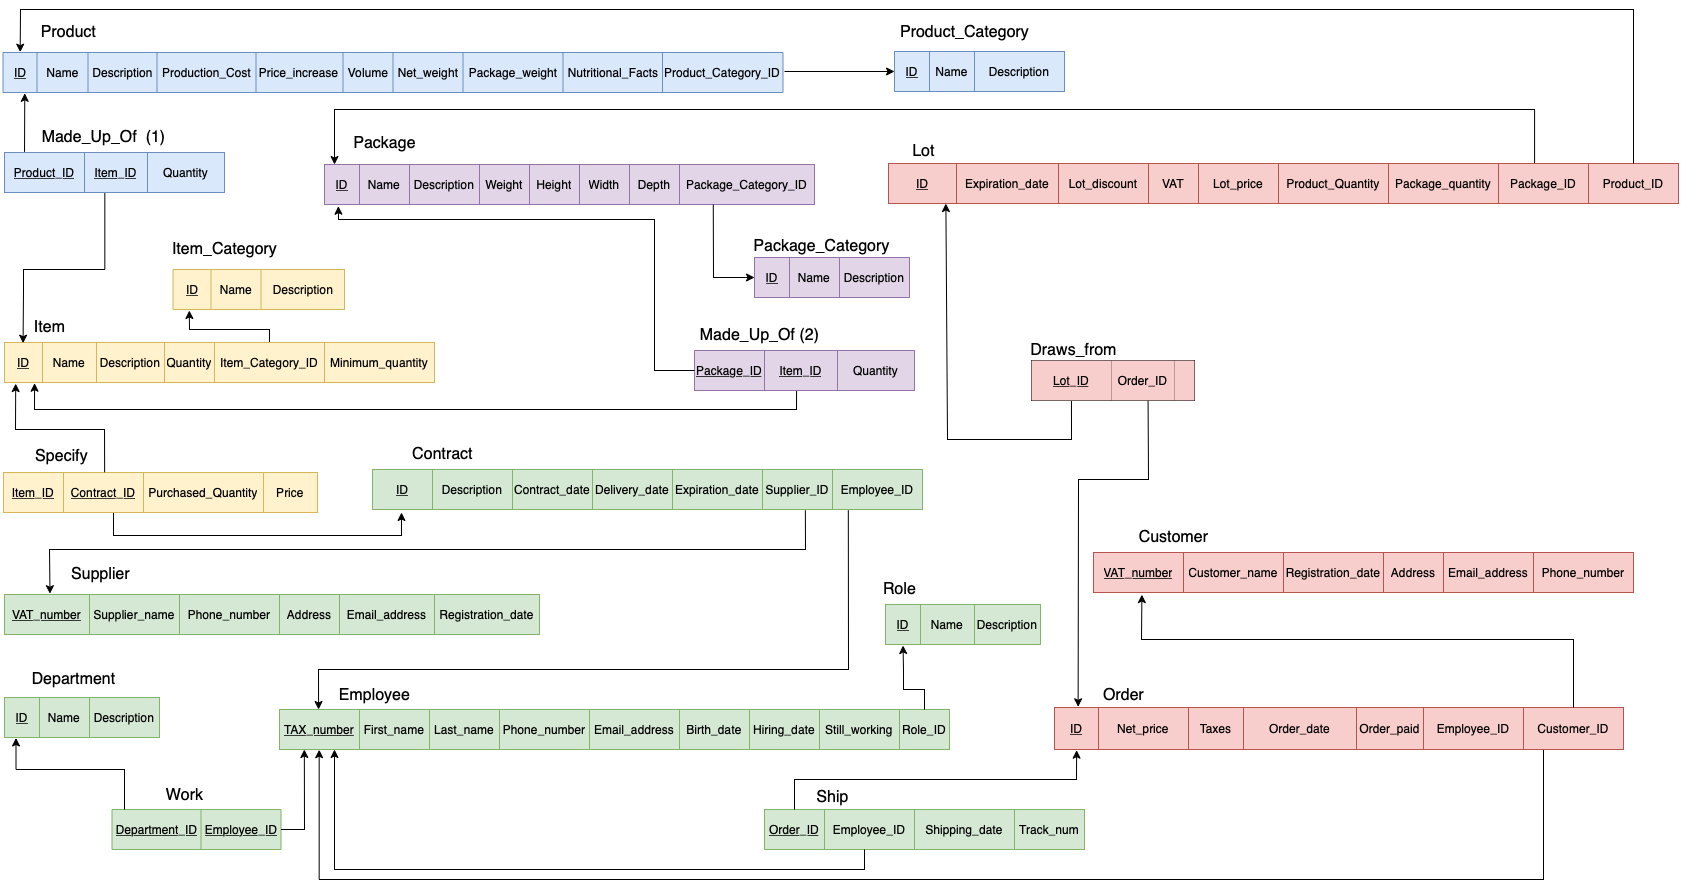
\includegraphics[width=1.3\linewidth,angle=270,origin=c]{Relational.png}
	\caption{Relational schema.}
	\label{fig:relational-schema}
\end{figure}
\newgeometry{margin=25mm}
Ship is a one to many relationship with optional participation, we decided to create Ship relation instead of using a foreign key in Order relation that refers to the Employee that ships the order. By this way we avoid having NULL values in the orders that have not been shipped yet in Order.
Draws from is a one to many relationship with optional participation. In this case, we also decided to create Draws relation and avoid having NULL  values in the lots that are ready but still haven't been ordered in Lot relation.
